\setcounter{section}{10}
\section{Сортировки. Доказательство логарифмической формулы}
\noindent Пусть даны объекты $a_1, \ldots, a_n$ с отношением порядка и их необходимо отсортировать по возрастанию (нестрого).
\\ \par \textbf{Лемма: } $\log{n!}=\Theta(n\log{n})$
$$\blacktriangle \qquad \log{n!}=\log{1}+\log{2}+\ldots+\log{n} \leq n\log{n} \Rightarrow \log{n!}=O(n\log{n})$$
$$\log{n!} \geq \frac{n}{2}\cdot \log{\frac{n}{2}} = \frac{n}{2}(\log{n} - \log{2}) = \frac{1}{2}n\log{n} - \frac{1}{2}n\log{2} \Rightarrow \log{n!}=\Omega(n\log{n})$$
Следовательно, $\log{n!}=\Theta(n\log{n})$ \quad $\blacksquare$

\par \textbf{Определение: } Сортировка называется \textit{устойчивой}, если она не меняет порядок равных с точки зрения операции сравнения элементов.

\section{Сортировки. Нижняя оценка на число сравнений в сортировке сравнениями}
\textbf{Теорема (Нижняя оценка на число сравнений в сортировке сравнениями)} Пусть единственное, что можно делать с объектами - это их сравнивать, тогда для сортировки в худшем случае потребуется $\Omega(n\log{n})$ сравнений.

\par $\blacktriangle$ Задача состоит в поиске одной из $n!$ перестановок. Заметим, что при ответе на запрос: какое из двух чисел должно стоять раньше? - количество перестановок уменьшается в два раза. То есть $n! \mapsto \frac{n!}{2} \mapsto \frac{n!}{4} \mapsto \ldots \;$, что влечет хотя бы $\log{n!}$ итераций $\Rightarrow$ (по лемме) $\Omega(n\log{n})$.  \quad $\blacksquare$

\setcounter{section}{12}
\section{Сортировка слиянием (Merge Sort)}

\par \textbf{Принцип работы: } Алгоритм использует принцип «разделяй и властвуй»: задача разбивается на подзадачи меньшего размера, которые решаются по отдельности, после чего их решения комбинируются для получения решения исходной задачи. Конкретно процедуру сортировки слиянием можно описать следующим образом:

\begin{enumerate}
    \item Если в рассматриваемом массиве один элемент, то он уже отсортирован — алгоритм завершает работу.
    \item Иначе массив разбивается на две части, которые сортируются рекурсивно.
    \item После сортировки двух частей массива к ним применяется процедура слияния, которая по двум отсортированным частям получает исходный отсортированный массив.
\end{enumerate}
У нас есть два массива $a$ и $b$ (фактически это будут две части одного массива, но для удобства будем писать, что у нас просто два массива). Нам надо получить массив $c$ размером $|a|+|b|$. Для этого можно применить процедуру слияния. Эта процедура заключается в том, что мы сравниваем элементы массивов (начиная с начала) и меньший из них записываем в финальный. И затем, в массиве у которого оказался меньший элемент, переходим к следующему элементу и сравниваем теперь его. В конце, если один из массивов закончился, мы просто дописываем в финальный другой массив. После мы наш финальный массив записываем заместо двух исходных и получаем отсортированный участок.
\newline \newline \textbf{Достоинства: } устойчивая и можно написать эффективную многопоточную сортировку слиянием.
\newline \textbf{Недостатки: } требуется дополнительно $O(n)$ памяти, но можно модифицировать до $O(1)$.

\newpage 
Ниже приведён псевдокод процедуры слияния двух частей массива $a$ — $[left;mid)$ и $[mid;right)$
\begin{figure}[h]
\centering
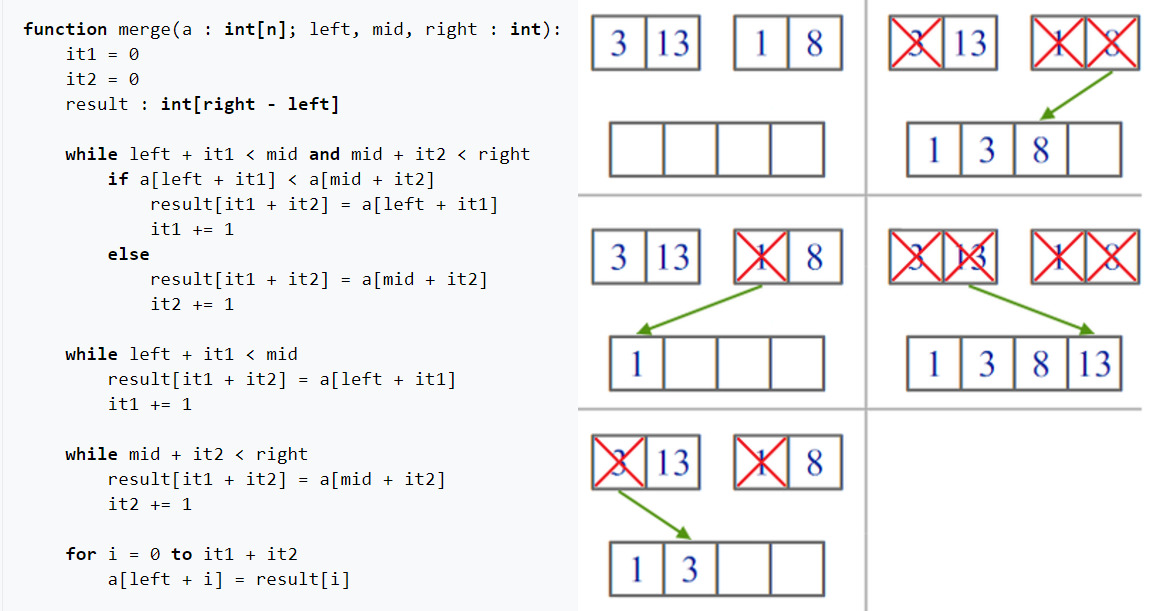
\includegraphics[width=1\linewidth]{images/13_pic1.jpg}
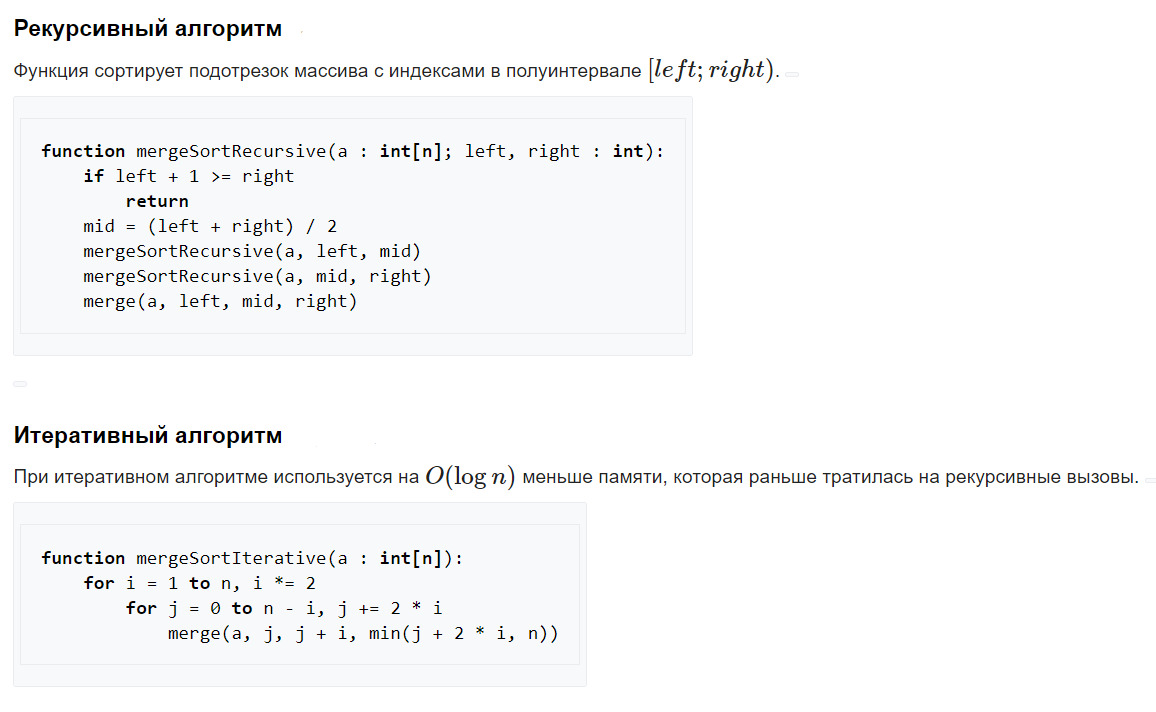
\includegraphics[width=1\linewidth]{images/13_pic3.jpg}
\end{figure}
\par Чтобы оценить \textbf{время работы} этого алгоритма, составим рекуррентное соотношение. Пускай $T(n)$ — время сортировки массива длины $n$, тогда для сортировки слиянием справедливо $T(n)=2T(n/2)+O(n)$, где $O(n)$ — время, необходимое на то, чтобы слить два массива длины $n$. Распишем это соотношение:
$$T(n)=2T(\frac{n}{2})+O(n)=4T(\frac{n}{4})+2\cdot O(n)=\ldots=T(1)+\log{n}O(n)=O(n\log{n})$$

\newpage \setcounter{section}{13}
\section{Поиск числа инверсий в массиве}
\noindent Пусть даны объекты $a_1, \ldots, a_n$. Тогда пара $(i,j)$ образует инверсию, если $i<j$ и $a_i>a_j$.
\newline Пусть $F(A)$ - число инверсий в массиве $A$. Тогда $F(A)=F(B)+F(C)+\#(p,t) : B_p>B_t$
\newline Для решения этой задачи нам подойдет сортировка слиянием, потому что при ее реализации мы знаем из какого массива приходит число, а следовательно и можем посчитать инверсии. Значит \textbf{время работы} этого алгоритма составит $O(n\log{n})$.
\\ \par \textbf{Подсчет инверсий} происходит следующим образом: если в обоих сливаемых массивах есть элементы, то каждый раз когда элемент берётся из массива $C$ к количеству инверсий нужно прибавлять количество элементов оставшихся в массиве $B$.

\setcounter{section}{14}
\section{Быстрая сортировка (Quick Sort). Лемма о частичной сумме гармонического ряда}

\noindent Быстрый метод сортировки функционирует по принципу "разделяй и властвуй":
\begin{itemize}
    \item Массив $a[l, \ldots, r]$ типа $T$ разбивается на два (возможно пустых) подмассива $a[l, \ldots, p]$ и $a[p+1, \ldots, r]$ ($p$ = pivot), таких, что каждый элемент $a[l, \ldots, p]$ меньше или равен $a[m]$, который в свою очередь, не превышает любой элемент подмассива $a[p+1, \ldots, r]$. Индекс вычисляется в ходе процедуры разбиения.
    \item Подмассивы $a[l, \ldots, p]$ и $a[p+1, \ldots, r]$ сортируются с помощью рекурсивного вызова процедуры быстрой сортировки.
    \item Поскольку подмассивы сортируются на месте, для их объединения не требуются никакие действия: весь массив $a[l, \ldots, r]$ оказывается отсортированным.
\end{itemize}
Процедура partition, которая переставляет элементы массива $a[l, \ldots, r]$ типа $T$ нужным образом, работает за $\Theta(n)$. Прежде всего, в качестве разделяющего элемента произвольно выбирается pivot = $a_i$, где $i$ - случайный индекс. Далее начинается просмотр с левого конца массива, который продолжается до тех пор, пока не будет найден элемент, превосходящий по значению разделяющий элемент, аналогично с правого конца массива до тех пор, пока не отыскивается элемент, который по значению меньше разделяющего. Оба элемента, на которых просмотр был прерван, очевидно, находятся не на своих местах в разделенном массиве, и потому они меняются местами. Так продолжаем дальше, пока указатели не встретяться.

\textbf{Достоинства: } 
\begin{itemize}
    \item Требует лишь $O(\log n)$ дополнительной памяти для своей работы. (Не улучшенный рекурсивный алгоритм в худшем случае $O(n)$ памяти)
    \item Хорошо сочетается с механизмами кэширования
\end{itemize}
\textbf{Недостатки: } 
\begin{itemize}
    \item Сильно деградирует по скорости (до $O(n^2)$) в худшем или близком к нему случае, что может случиться при неудачных входных данных.
    \item Рекурсивная реализация может привести к ошибке переполнения стека, так как в худшем случае может потребоваться сделать $O(n)$ вложенных рекурсивных вызовов.
    \item Неустойчивая сортировка
\end{itemize}

\par \textbf{Лемма: } $S_n = 1+\frac{1}{2}+\frac{1}{3}+\ldots+\frac{1}{n}=\Theta(\log{n})$

$\blacktriangle$ Пусть $2^k$ - минимальная степень двойки, такая что $2^k\leq n \Rightarrow k = [\log_2{n}]$ 
$$ S_n \geq S_{2^k} = 1 + \frac{1}{2} + \underbrace{\frac{1}{3}+\frac{1}{4}}_{\geq \frac{1}{2}}+ \underbrace{\frac{1}{5}+\frac{1}{6}+ \frac{1}{7} + \frac{1}{8}}_{\geq \frac{1}{2}} + \ldots + \frac{1}{2^k}\geq \frac{1}{2}\cdot \log{2^k} = \frac{k}{2} \Rightarrow S_n=\Omega(\log{n})$$

Пусть $2^m \geq n$, такая что $m = [\log_2{n}]$
$$ S_n \leq S_{2^m} = 1 + \frac{1}{2} + \underbrace{\frac{1}{3}+\frac{1}{4}}_{\leq 1}+ \underbrace{\frac{1}{5}+\frac{1}{6}+ \frac{1}{7} + \frac{1}{8}}_{\leq 1} + \ldots + \frac{1}{2^m}\leq 1\cdot m = m \Rightarrow S_n=O(\log{n})$$

Следовательно, $S_n=\Theta(\log{n})$ \quad $\blacksquare$

\section{Быстрая сортировка (Quick Sort). Доказательство времени работы при случайном выборе пивота. }

\par \textbf{Время работы} этого алгоритма пропорционально числу сравнений. Обозначим через $D$ — массив $A$ после сортировки, то есть $D_1\leq D_2\leq \ldots \leq D_n$. Вопрос: с какой вероятностью $D_i$ и $D_j$ ($i<j$) будут когда-либо сравниваться в алгоритме? \newline Ответ: если на каком-то шаге 
\begin{itemize}
    \item pivot > $D_j$ или pivot < $D_i$, то $D_i$ и $D_j$ еще не сравнились, но в будущем у них есть шанс сравниться;
    \item $D_i$ < pivot < $D_j$, то $D_i$ и $D_j$ точно никогда не сравняться;
    \item pivot = $D_j$ или pivot = $D_i$, то $D_i$ и $D_j$ сравнятся со всеми и в частности друг с другом;
\end{itemize}
Следовательно, сравнение происходит, если среди элементов $D_i , D+{i+1}, \ldots , D_j$ первым в качесте пивота выбран один из крайних элементов. Поэтому вероятноть равна $\frac{2}{j-i+1}$. Пусть $k=j-i+1$
$$\mathbb{E}T(n) \sim \sum_{i<j}\frac{2}{j-i+1}=\sum_{k=2}^{n}\frac{2}{k}\cdot (n-k+1)\leq \sum_{k=2}^{n}\frac{2}{k}\cdot n \Rightarrow O(n\log n)$$

\par \textbf{Худшее время работы}
\newline Предположим, что мы разбиваем массив так, что одна часть содержит $n-1$ элементов, а вторая — 1. Поскольку процедура разбиения занимает время $\Theta(n)$, для времени работы $T(n)$ получаем соотношение:
$$T(n)=T(n-1)+\Theta(n)=\sum_{k=1}^{n}\Theta(k)=\Theta(\sum_{k=1}^{n}k)=\Theta(n^2)$$
Значит при максимально несбалансированном разбиении время работы составляет $\Theta(n^2)$. В частности, это происходит, если массив изначально отсортирован.